\chapter{熱史、最終散乱、そして原始スープ}

\lectureoverview{宇宙の膨張史は熱史でもある。まず温度を平衡によって定義し、平衡を散乱によって定義する。自由電荷が光子気体を熱平衡に保つ間、光子気体はプランクスペクトルを獲得する。電子が陽子に束縛されると放射は脱結合するが、すべての波長がスケール因子とともに伸びるため、黒体の形は保たれる。すると光子対物質の膨大な比が、なぜ再結合が水素の電離温度よりはるかに低いところで起こるかを説明する。さらに過去へさかのぼると、最終散乱、物質--放射の等量、電子--陽電子対の平衡、そして対消滅を生き延びたわずかな物質--反物質の超過へと至る。}

\section{モデルフィッティングから熱史へ}

宇宙論的モデルは、最低限、スケール因子の履歴と空間幾何によって指定される。
\begin{equation}
a(t),
\qquad
k\in\{+1,0,-1\}.
\end{equation}
実用的な方法は、モデルを選び、それが予言するものを計算し、それらの予言をデータと比較し、パラメータを調整することである。データから直接推論を逆向きに走らせることも可能だが、しばしば透明性に欠ける。

曲率を比較的近傍の源から決定するのは難しい。地球の曲率が短い地上基線では小さな補正にすぎないのと同様に、宇宙論的基線が十分大きくなければ空間曲率は弱い効果である。これは欠点であると同時に利点でもある。通常の源サーベイは\(k\)を鋭く決定しないが、\(k\)の適度な不確かさは膨張史の有用な再構成を妨げない。

二つの観測量の系列がその大半を担う。標準光源は赤方偏移の関数としての明るさを与え、源サーベイは赤方偏移区間内の天体数を与える。得られるフィットは、かなりの真空エネルギー寄与を含む膨張史を支持する。精密な曲率情報には、宇宙マイクロ波背景放射が与えるはるかに長い幾何学的てこの腕が必要である。

ここで問いを変える。\(a(t)\)がどのように進化するかだけを問うのではなく、宇宙の温度がどのように進化するかを問うのである。その問いは、より初歩的な問いから始まる。すなわち、系がそもそも温度をもつのはどのような条件のもとでか、である。

\section{宇宙が温度をもつとき}

温度は熱平衡の性質である。粒子の集まりは衝突を通じて平衡に近づき、それらの衝突は巨視的な環境が変化するよりも速く働かなければならない。膨張宇宙では有用な比較は
\begin{equation}
\tau_{\rm scatt}\ll H^{-1},
\label{eq:c07-equilibrium-condition}
\end{equation}
であり、ここで\(\tau_{\rm scatt}\)は特徴的な散乱時間、\(H^{-1}\)は膨張時間である。この不等式が成り立たないとき、衝突が平衡を回復する前に宇宙が変化してしまう。

完全反射の箱を考える。レーザーパルスをその中に照射し、開口部を閉じ、箱には光子しか含まれていないと仮定する。パルスは無限に跳ね返るが、通常の低エネルギー光子は互いにきわめて弱くしか散乱しない。反射だけではそれらのエネルギーを熱スペクトルへ再分配しない。したがって光子気体は、閉じ込められているというだけでは熱平衡化しない。

自由な荷電粒子は状況を変える。電磁波は電子を加速し、加速された電荷は再放射するので、光子は効率よく散乱する。十分な自由電子と陽子があれば、繰り返しの散乱が三種すべての間でエネルギーを再分配し、それらは共通の温度をもつ一つの熱いスープを形成する。

大きなスケールでは宇宙は電気的に中性である。最も単純な記帳では、
\begin{equation}
n_{e^-}=n_p,
\label{eq:c07-neutrality}
\end{equation}
となる。電子と陽子の電荷は大きさが等しく符号が反対だからである。この式は中性を述べているのであって、なぜ電荷が中性なのか、なぜ二つの電荷の大きさが一致するのかを説明するものではない。それらは素粒子物理学に関するより深い事実である。

プラズマと中性気体の区別は決定的である。自由電子は放射を効率よく散乱する。電子が陽子に束縛されて中性水素をつくると、支配的な電場は長距離で打ち消し合い、散乱ははるかに効かなくなる。現在の宇宙の低密度では、中性物質は宇宙の寿命のうちに背景光子を平衡へもたらすことができない。

十分高い温度では、高エネルギーの衝突が水素を繰り返し電離し、自由電荷のかなりの集団を維持する。そのとき電子、陽子、光子は一つの温度を共有する。系が冷えるにつれて原子が生き残り、自由電子密度が崩壊し、共通の平衡は失われる。その後、物質と放射に割り当てられる温度は一致する必要がない。

\begin{classroomqa}
\audiencequestion{マイクロ波背景放射の温度が\(3\,\mathrm{K}\)付近にあるなら、それは今日の宇宙全体の温度なのか。}
\lecturerresponse{いいえ。光子スペクトルは黒体温度でラベル付けできるが、現在の物質はそれら光子と平衡にはない。異なる成分は異なる運動温度または有効温度をもつので、今日、単一の大域的な熱力学的温度は存在しない。}
\end{classroomqa}

\section{熱放射と量子への転換}

平衡放射場は、
\begin{equation}
\nu\lambda=c.
\end{equation}
で関係づけられる波長と振動数のスペクトルを含む。放射輝度とエネルギー密度を混同しないために、\(u_\nu(T)\)を単位振動数あたり、単位体積あたりのエネルギーを表すものとしよう。
\begin{equation}
dE=u_\nu(T)\,dV\,d\nu.
\label{eq:c07-spectral-density}
\end{equation}
したがって\(u_\nu\)はエネルギーを体積と振動数で割った次元をもつ。

温度それ自体がエネルギーの尺度である。歴史的な温度の単位はその事実を覆い隠すので、ボルツマン定数が換算を与える。
\begin{equation}
E_{\rm thermal}\sim k_B T.
\end{equation}
自然単位で\(k_B=1\)と置いてもよいが、それを保持すればケルビンとエネルギーが目に見えて区別されたままになる。

量子力学以前には、\(k_BT\)、\(\nu\)、\(c\)を用いた次元解析からレイリー--ジーンズのスペクトルエネルギー密度
\begin{equation}
u_\nu^{\rm RJ}(T)=\frac{8\pi\nu^2}{c^3}k_BT.
\label{eq:c07-rayleigh-jeans}
\end{equation}
が得られる。数値因子は電磁モードの数え方に依存するが、本質的な古典的振る舞いは\(u_\nu\propto T\nu^2\)である。それは振動数が増すにつれて際限なく増大し、したがって
\begin{equation}
\int_0^\infty u_\nu^{\rm RJ}\,d\nu=\infty.
\end{equation}
を予言する。この不可能な結果が紫外発散である。測定されたスペクトルは代わりに増大し、転回し、有限のエネルギーを含むのに十分な速さで減少する。

プランク定数が欠けていた量子スケールを導入する。式~\eqref{eq:c07-spectral-density}で定義されたスペクトルエネルギー密度に対して、プランクの法則は
\begin{equation}
u_\nu(T)
=
\frac{8\pi h\nu^3}{c^3}
\frac{1}{e^{h\nu/(k_BT)}-1}.
\label{eq:c07-planck}
\end{equation}
である。指数は無次元比
\begin{equation}
x=\frac{h\nu}{k_BT},
\end{equation}
に依存する。なぜなら\(E_\gamma=h\nu\)と\(k_BT\)はどちらもエネルギーだからである。

低振動数では\(x\ll1\)であり、
\begin{equation}
e^x-1=x+O(x^2).
\end{equation}
である。式~\eqref{eq:c07-planck}に代入すると
\begin{align}
u_\nu(T)
&\simeq
\frac{8\pi h\nu^3}{c^3}
\frac{k_BT}{h\nu}
\\
&=
\frac{8\pi\nu^2}{c^3}k_BT,
\end{align}
となるので、古典物理学はその適切な低振動数の領域で回復される。高振動数では\(x\gg1\)であり、指数関数が支配してスペクトルを抑え込む。移行は
\begin{equation}
\frac{h\nu}{k_BT}\sim1.
\label{eq:c07-crossover}
\end{equation}
で起こる。これが量子への転換が古典的増大を置き換える点である。

\begin{figure}[htbp]
\centering
\includegraphics[width=0.82\textwidth]{lecture_07_figure_02.png}
\caption{黒板上の熱的転換。切り取られた上の式は\(h\nu/(kT)>1\)であり、はっきり見える下の式は\(hc/(kT)>\lambda\)である。下の黒板のかすかな残りは方程式の証拠としては用いない。}
\label{fig:c07-thermal-board}
\lectureframe{00:44:42.840}
\end{figure}

\(\nu=c/\lambda\)を用いると、転換は桁程度の熱的波長
\begin{equation}
\boxed{\lambda_{\rm th}\sim\frac{hc}{k_BT}}.
\label{eq:c07-thermal-wavelength}
\end{equation}
を定義する。より短い波長は指数関数的に抑えられた裾にあり、パワーの大部分はこの程度の波長によって運ばれる。ただし数値因子は、スペクトルを単位振動数あたりで描くか単位波長あたりで描くかに依存する。

\begin{classroomqa}
\audiencequestion{プランクはここで用いた電子--陽子プラズマ模型からスペクトルを得たのか。}
\lecturerresponse{いいえ。彼は経験的なスペクトル情報をウィーンの変位則と組み合わせた。それはすでに、ピーク波長が温度に反比例して変化することを示していた。そのスケーリングが新しい定数\(h\)を明らかにした。プランクはその結果を物質の壁の中の振動子と結びつけたが、放射場の完全な量子的解釈は後にもたらされた。\lecturetimestamp{00:37:06--00:39:25}}
\end{classroomqa}

\begin{classroomqa}
\audiencequestion{なぜ次元の検査は\(c\)の1乗を見落としているように見えたのか。}
\lecturerresponse{最初に強度と呼ばれた量は、単位振動数あたり、単位体積あたりのエネルギーとして定義されていたが、\(2h\nu^3/c^2\)を含むよく知られた式は、単位面積、単位立体角あたりの分光放射輝度である。スペクトルエネルギー密度は\(c^{-3}\)と角度因子を伴う。式~\eqref{eq:c07-planck}のように。この修正は規格化の慣習を変えるのであって、無次元比\(h\nu/(k_BT)\)や熱的波長を変えるのではない。\lecturetimestamp{00:39:33--00:44:51}}
\end{classroomqa}

その規格化を別にすれば、プランクスペクトルは普遍的な形をもつ。式~\eqref{eq:c07-planck}は
\begin{equation}
u_\nu(T)=T^3\,F\!\left(\frac{\nu}{T}\right),
\label{eq:c07-scaling-form}
\end{equation}
と書ける。ただし定数は\(F\)に吸収されている。\(T\)を上げると振動数軸と全体の高さが再スケールされ、同じ無次元曲線が再び現れる。波長の言葉では、温度を上げるとスペクトルはより短い波長へと圧縮される。

\begin{figure}[htbp]
\centering
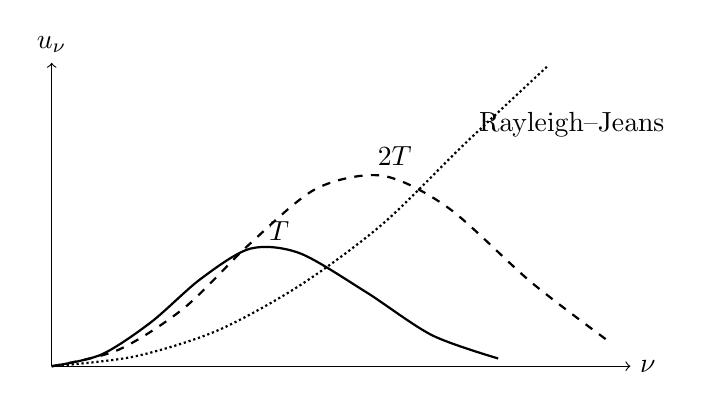
\begin{tikzpicture}[x=1.05cm,y=0.82cm]
\draw[->] (0,0)--(7.0,0) node[right] {\(\nu\)};
\draw[->] (0,0)--(0,4.7) node[above] {\(u_\nu\)};
\draw[densely dotted,thick] plot[smooth] coordinates
  {(0,0) (1,0.15) (2,0.55) (3,1.25) (4,2.20) (5,3.45) (6,4.65)};
\draw[thick] plot[smooth] coordinates
  {(0,0) (0.6,0.18) (1.2,0.68) (1.8,1.35) (2.4,1.82) (3.0,1.75) (3.8,1.15) (4.6,0.48) (5.4,0.12)};
\draw[thick,dashed] plot[smooth] coordinates
  {(0,0) (0.8,0.25) (1.6,0.90) (2.4,1.90) (3.2,2.75) (4.0,2.95) (4.8,2.45) (5.8,1.30) (6.7,0.42)};
\node[anchor=west] at (5.05,3.75) {Rayleigh--Jeans};
\node at (2.75,2.10) {\(T\)};
\node at (4.15,3.25) {\(2T\)};
\end{tikzpicture}
\caption{古典的スペクトルは際限なく増大するが、プランクスペクトルは転回する。温度を上げると特徴的な振動数は上方へ移り、無次元の形は保たれる。}
\label{fig:c07-planck-redraw}
\end{figure}

現在の宇宙に存在する光子の圧倒的多数はマイクロ波背景放射に属し、その特徴的な波長はおよそ一ミリメートルである。式~\eqref{eq:c07-thermal-wavelength}はその波長を数ケルビンと結び付け、ここでは慣例に従って\(3\,\mathrm{K}\)に丸めている。波長だけでは大まかな関連しか与えられない。より強い証拠は、多数の周波数にわたる測定が完全な黒体曲線を極めて高い精度でなぞることである。

\begin{classroomqa}
\audiencequestion{マイクロ波背景放射の光子一つはどれだけの空間を占めるのか。}
\lecturerresponse{光子には普遍的な硬い境界の大きさはない。光子は状態に依存する空間的広がりをもつ波束として用意されうる一方、その波長が振動の尺度を定める。熱的背景では、特徴的な波長と自然な波束の尺度はいずれもおよそ一ミリメートルであるが、どちらも小さな古典的物体の半径と取り違えてはならない。\lecturetimestamp{00:57:16--00:59:05}}
\end{classroomqa}

\section{膨張が黒体の形を凍結する}

電離した水素と放射が平衡にある高温の箱から始める。箱が膨張するにつれて、その内容物は仕事をし、エネルギー密度は低下し、温度は減少する。やがて電子と陽子は中性原子として束縛されたままになる。原子の形成は\emph{再結合}と呼ばれ、効率的な光子--物質散乱の喪失は\emph{脱結合}と呼ばれる。この二つの過程は密接に関連しているが、異なる物理的出来事を名指している。

脱結合後、物質と放射はもはや共通の温度を共有しない。それでも光子スペクトルはそのプランク形を保つ。自由に伝播するすべての波長は同じ膨張因子によって引き伸ばされる。
\begin{equation}
\lambda\propto a,
\qquad
\nu\propto a^{-1}.
\end{equation}
プランク曲線は\(\nu/T\)に依存するので、この一様な赤方偏移は放射に温度を割り当てることと等価である。
\begin{equation}
\boxed{T_\gamma\propto a^{-1}.}
\label{eq:c07-temperature-scaling}
\end{equation}
したがって膨張は、衝突が絶えずそれを再構築することなくても、その形を保存する。物質はその後、独自の熱史をたどる。

したがって観測されるマイクロ波背景放射は、化石的な平衡分布である。その黒体形は自由電荷が効率的に散乱していた間に確立され、その後は一様な宇宙論的赤方偏移によって引き継がれた。星の光、ガンマ線、その他の後期の源も存在するが、それらは残存光子集団に比べて数的に小さく、同定可能な天体物理的起源を持つ。

\begin{classroomqa}
\audiencequestion{放射がもはや物質と平衡にない後でも、なぜ黒体のままでいられるのか。}
\lecturerresponse{平衡スペクトルを創り出すには衝突が必要だが、完全に一様な膨張の下でそれを保存するには必要ない。すべての波長に同じ因子を掛けることは、一つのプランクスペクトルをより低い温度の別のプランクスペクトルに写す。光子は物質の温度を共有することをやめるが、それ自身の黒体温度は保つ。}
\end{classroomqa}

\section{なぜ再結合はそれほど遅く起こるのか}

今日の波長と脱結合時の波長は次で関係づけられる。
\begin{equation}
\frac{\lambda_0}{\lambda_{\rm dec}}
=
\frac{a_0}{a_{\rm dec}}
=
\frac{T_{\rm dec}}{T_0}.
\label{eq:c07-decoupling-ratio}
\end{equation}
脱結合は数学的に瞬時ではないが、その後の歴史と比べて十分短いので、特徴的なスケール因子と温度を割り当てることができる。ここで\(T_0\)はCMB温度を意味し、銀河間物質の運動温度ではない。

水素の基底状態の電離エネルギーは
\begin{equation}
\chi_H=13.6\,\mathrm{eV}.
\end{equation}
最初の推測では\(k_BT\sim\chi_H\)と置き、典型的な光子が原子を電離できるとするだろう。その推測ははるかに高すぎる。なぜなら熱スペクトルは高エネルギー側の裾を含み、宇宙は膨大な数の光子を含むからである。

\begin{figure}[htbp]
\centering
\includegraphics[width=0.82\textwidth]{lecture_07_figure_03.png}
\caption{黒板は観測された存在比\(N_\gamma/N_e=10^8\)と光子エネルギーの記号\(\epsilon\)を導入している。指数関数の始まりだけが見えており、完成したボルツマン因子は口頭の導出から続く。}
\label{fig:c07-boltzmann-board}
\lectureframe{01:06:10.631}
\end{figure}

ここで用いる丸めた存在比は
\begin{equation}
\frac{N_\gamma}{N_e}\sim10^8.
\label{eq:c07-photon-electron-ratio}
\end{equation}
である。これは測定されたCMB光子密度を通常物質の目録と比較することによって推論される。光子エネルギー\(\epsilon\)に対して、高エネルギー側の裾はボルツマン形
\begin{equation}
P(\epsilon)\propto e^{-\epsilon/(k_BT)}.
\end{equation}
をとる。したがって、原子あたりに利用可能な電離光子の数は
\begin{equation}
10^8 e^{-\chi_H/(k_BT)}.
\end{equation}
によって見積もられる。電離はこの量が一の程度にまで下がるまで有効であり続ける。

対数を取ると
\begin{equation}
\frac{\chi_H}{k_BT}
\sim
\ln 10^8
\simeq18.4,
\end{equation}
あるいは、意図された精度では
\begin{equation}
k_BT\sim\frac{\chi_H}{20}.
\label{eq:c07-tail-estimate}
\end{equation}
特徴的な光子は閾値よりはるかに低くてもよい。なぜなら裾からの電離光子1個が各原子に対して十分だからである。

\begin{classroomqa}
\audiencequestion{尾部の見積もりは、しきい値ちょうどの光子を数えるのか、それともそれより上のすべての光子を数えるのか。}
\lecturerresponse{しきい値以上、すなわちしきい値ちょうどとそれより上の光子を数える。尾部は指数関数的に減少するので、その積分の大部分は\(\chi_H\)付近のエネルギーから寄与し、したがって単純な指数関数的見積もりで関連する桁を捉えられる。\lecturetimestamp{01:08:39--01:08:54}}
\end{classroomqa}

\begin{classroomqa}
\audiencequestion{脱結合の時点でも比\(N_\gamma/N_e\)はおよそ\(10^8\)だったのか。}
\lecturerresponse{ここで用いた近似の範囲では、そのとおりである。脱結合からかなり高温の時代にさかのぼるまで、膨張は両方の集団を同じ体積因子で希釈し、どちらの種もその比を変えるほどには生成も消滅もさせない。さらに高温では、対生成反応に新たな勘定が必要になる。\lecturetimestamp{01:08:54--01:09:57}}
\end{classroomqa}

\begin{classroomqa}
\audiencequestion{恒星から放出された光子はこの数に無視できない寄与をするのか。}
\lecturerresponse{しない。再結合の時点では恒星はまだ存在せず、今日でも恒星の光子は宇宙マイクロ波背景放射の集団のごく一部にすぎない。式~\eqref{eq:c07-photon-electron-ratio}の比は遺存熱的光子に関するものである。\lecturetimestamp{01:11:44--01:12:39}}
\end{classroomqa}

\begin{classroomqa}
\audiencequestion{電子が陽子と再結合するとき、放出された光子は黒体スペクトルに鋭い水素の特徴を残すべきか。}
\lecturerresponse{散乱と吸収が膨張に比べて速いままであれば、放射は絶えず再処理され、熱平衡に近いままである。十分に急激な凍結が起これば歪みが保存されうるが、平衡に近い緩やかな再結合では、大きな孤立した線が黒体の形を置き換えることはない。\lecturetimestamp{01:12:42--01:14:07}}
\end{classroomqa}

その結果得られる教室での見積もりは\(T_{\rm dec}\sim4\times10^3\,\mathrm{K}\)である。\(\chi_H/20\)を直接換算するとやや高い値が得られ、有効な分母は\(40\)に近いかもしれないという示唆につながる。これは矛盾ではなく、完全な電離平衡を一つの尾部の数え上げで置き換えることの粗さを露呈している。制御された平衡の取り扱いではサハの関係式
\begin{equation}
\frac{x_e^2}{1-x_e}
=
\frac{1}{n_H}
\left(\frac{m_e k_BT}{2\pi\hbar^2}\right)^{3/2}
e^{-\chi_H/(k_BT)},
\label{eq:c07-saha}
\end{equation}
を用い、続いて非平衡の再結合動力学を扱う。この粗い議論は、支配的な物理を特定するという点で価値がある。すなわち、ごく小さいバリオン対光子比が、中性原子の生存を\(\chi_H/k_B\)よりはるかに低い温度まで遅らせるのである。

\section{最終散乱面への赤方偏移}

\(T_0\simeq3\,\mathrm{K}\)および\(T_{\rm dec}\sim4\times10^3\,\mathrm{K}\)を用いると、式~\eqref{eq:c07-decoupling-ratio}は
\begin{equation}
\boxed{
\frac{a_0}{a_{\rm dec}}
\sim
\frac{T_{\rm dec}}{T_0}
\sim10^3
}.
\label{eq:c07-decoupling-expansion}
\end{equation}
を与える。同等に、最終散乱の赤方偏移はおよそ\(10^3\)の桁である。この時代より前には、電離プラズマは不透明であった。その後、光子はほぼ自由に伝播した。

この熱的出来事は、高温膨張の始まりからわずか数十万年後に起こり、慣例的にこの対話ではおよそ\(380{,}000\)年と述べられている。その間隔は、その後の宇宙年齢に比べればごくわずかである。脱結合以来、長さはおよそ\(10^3\)倍に、共動体積要素はおよそ\(10^9\)倍に成長した。

脱結合は一つの熱的目印であり、その間の歴史における唯一の出来事ではない。銀河形成、恒星形成、ブラックホール形成はいずれもより後に起こるが、ここでは熱的目印をきれいにさかのぼって追えるようにするため、それらは脇に置く。

外を見ることは過去を見ることである。近くの殻は最近の時代を示し、より遠くの殻はより早い時代を示す。我々の過去光円錐はやがて再結合の時代に出会い、その時代との交わりが最終散乱面である。それより前の電磁放射は自由電荷によって繰り返し散乱され、我々に直接届くことはできなかった。

\begin{figure}[htbp]
\centering
\begin{coursefitfigure}
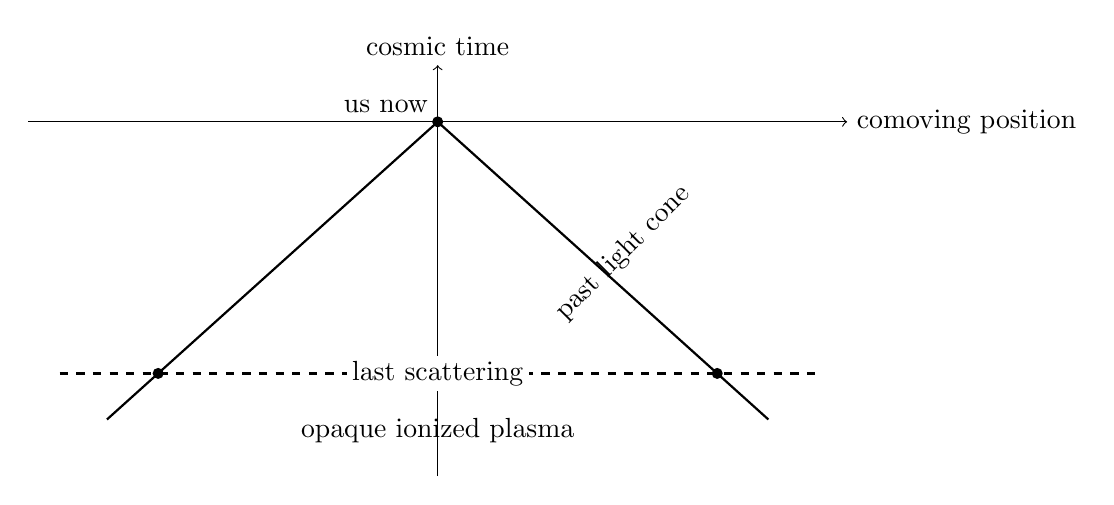
\begin{tikzpicture}[x=1.0cm,y=0.9cm]
\draw[->] (0,0)--(0,5.8) node[above] {cosmic time};
\draw[->] (-5.2,5.0)--(5.2,5.0) node[right] {comoving position};
\draw[thick] (0,5.0)--(-4.2,0.8);
\draw[thick] (0,5.0)--(4.2,0.8);
\draw[thick,dashed] (-4.8,1.45)--(4.8,1.45);
\fill (0,5.0) circle (2pt) node[above left] {us now};
\fill (-3.55,1.45) circle (2pt);
\fill (3.55,1.45) circle (2pt);
\node[fill=white,inner sep=2pt] at (0,1.45) {last scattering};
\node at (0,0.65) {opaque ionized plasma};
\node[rotate=45] at (2.35,3.15) {past light cone};
\end{tikzpicture}
\end{coursefitfigure}
\caption{電磁的観測は、過去光円錐に沿って最終散乱面までしかさかのぼれない。それより前の光子は電離プラズマによって繰り返し散乱された。}
\label{fig:c07-last-scattering}
\end{figure}

\begin{classroomqa}
\audiencequestion{脱結合は、それより早い時代のあらゆる可能な観測を終わらせるのか。}
\lecturerresponse{プラズマが光子に対して不透明であったため、直接の電磁的観測は終わる。より弱く相互作用する使者はそれより早く逃れうる。遺存ニュートリノは原理的により深い層を探り、重力放射はさらに早い情報を運びうる。したがって、最終散乱面より先についての我々の知識の多くは間接的であるが、恣意的ではない。\lecturetimestamp{01:32:27--01:36:31}}
\end{classroomqa}

\begin{classroomqa}
\audiencequestion{最初に\(a\)の絶対値はいくらであったのか、そして宇宙は必然的に小さな有限の物体であったのか。}
\lecturerresponse{平坦空間ではスケール因子の比のみが不変な意味を持ち、\(a\)の規格化は任意である。負の曲率を持つ空間的断面も無限でありうる。閉じた\(k=+1\)宇宙は有限の曲率半径を持つが、観測が決めるのは依然として膨張の比であって、既知の原始的な大きさではない。熱いビッグバンとは、それ自体で、すべての空間が小さな球であったという主張ではない。\lecturetimestamp{01:30:05--01:32:22}}
\end{classroomqa}

\begin{classroomqa}
\audiencequestion{CMBは銀河より古いので、それを見ることは、我々の観測可能な領域の外に今日銀河が存在するかどうかを教えてくれるのか。}
\lecturerresponse{いいえ。CMBは遠方の領域を脱結合時の姿として示すのであり、今日の姿として示すのではない。十分に大きな距離にある現在の銀河からの光は、我々に届く時間を持たなかった。我々の地平線の外に銀河の集団が引き続き存在することを支持するのは、観測された大規模な一様性と、可視の端が存在しないことであり、CMBが与える直接の眺めではない。\lecturetimestamp{01:59:01--02:00:58}}
\end{classroomqa}

その結果得られる時間軸は、現在から銀河形成と脱結合を経て物質--放射等量へと遡る。さらに以前では、収縮するスケール因子は温度の上昇と新たな粒子種の出現を意味する。

\section{物質--放射等量}

脱結合を越えて遡ると、もう一つの目印が現れる。非相対論的物質と放射は異なる仕方で薄まる：
\begin{equation}
\rho_m\propto a^{-3},
\qquad
\rho_r\propto a^{-4},
\qquad
\frac{\rho_m}{\rho_r}\propto a.
\label{eq:c07-equality-scaling}
\end{equation}
物質は遅い時期に支配するが、十分に小さい\(a\)では放射が必然的に支配する。膨張則はそれに対応して、物質時代の振る舞い\(a\propto t^{2/3}\)から放射時代の振る舞い\(a\propto t^{1/2}\)へと変わる。

意図的に粗い見積もりは、陽子あたり\(10^8\)個の光子、特徴的なCMB光子エネルギー\(10^{-4}\,\mathrm{eV}\)、陽子の静止エネルギー\(10^9\,\mathrm{eV}\)から出発する。暗黒物質を無視すると
\begin{equation}
\left(\frac{\rho_m}{\rho_r}\right)_0
\sim
\frac{10^9}{10^8\,10^{-4}}
\sim10^5.
\end{equation}
議論は次に自らを修正する：暗黒物質は発光するバリオンよりも実質的に多くの質量に寄与し、丸めた見積もりを\(10^6\)へと引き上げる。この算術の範囲内で、式~\eqref{eq:c07-equality-scaling}は等量を
\begin{equation}
\frac{a_{\rm eq}}{a_0}\sim10^{-6},
\qquad
\frac{T_{\rm eq}}{T_0}\sim10^6.
\label{eq:c07-equality-estimate}
\end{equation}
に置く。これらはスケールを定める教室での見積もりであり、精密な宇宙論的パラメータのフィットではない。その目的は、\(a\)の等しくない冪がどのように相次ぐ熱的时代を位置づけるかを示すことである。

放射支配時代は電磁的な最終散乱の壁の背後にあるが、その存在は測定された晩期の密度と既知のスケーリング則から従う。さらに高温へ進むと、陽子、電子、光子の数がそれぞれ固定されているという仮定はやがて無効になる。高エネルギーの衝突が重い粒子--反粒子対を生成し始めるからである。

\begin{classroomqa}
\audiencequestion{光子と陽子の数が保存されるという主張は、星の光と任意に高い温度を含むのか。}
\lecturerresponse{いいえ。それは、数を変える反応が効果的でない区間における残存CMB集団に当てはまる。星の光は後に作られたものであり、光子数において無視できる。十分に高い温度では、対生成が粒子の内容を変え、別々の数保存は破れる。再結合自体が加えるのは、電子あたりせいぜいおよそ1個の光子であり、既存のCMB集団のわずか\(10^8\)分の1にすぎない。\lecturetimestamp{01:26:24--01:27:40}}
\end{classroomqa}

\section{対生成とほぼ対称なスープ}

\begin{equation}
T\sim10^{10}\,\mathrm{K},
\qquad
\frac{a_0}{a}\sim10^{14},
\end{equation} 程度の温度では、特徴的な光子エネルギーは約一メガ電子ボルトであり、電子--陽電子対を生成するのに必要な静止エネルギー尺度に匹敵する。そのとき二つの光子は
\begin{equation}
\gamma+\gamma
\longleftrightarrow
e^-+e^+.
\label{eq:c07-pair-reaction}
\end{equation}
を通じて反応することができる。正確な閾値は衝突の運動学に依存するが、電子の静止エネルギー\(m_ec^2\)が関連する尺度を定める。

対生成と対消滅は急速に釣り合う。対が少なすぎれば、光子の衝突がそれらを補充し、対が多すぎれば、消滅がそのエネルギーを光子に戻す。したがって光子、電子、陽電子の存在量は温度によって決まり、相対論的プラズマ中ではすべて同程度の桁である。それらはもはや、後の数についての単純な記憶を保っていない。

\begin{classroomqa}
\audiencequestion{陽子と釣り合うのに必要な電子がすでにあるなら、この対で満たされたプラズマはどのようにして電気的に中性であり続けられるのか。}
\lecturerresponse{各反応は一つの負電荷と一つの正電荷を作るので、対は正味の電荷を加えない。それらは、わずかな電子の過剰の上に重ねられた、巨大でほぼ対称な集団である。個々の電子は区別できず、差\(N_{e^-}-N_{e^+}\)だけが、陽子と釣り合うのに必要な電荷を記憶している。\lecturetimestamp{01:42:31--01:43:14}}
\end{classroomqa}

対反応は和を変えるが差は保存する：
\begin{equation}
N_{e^-}+N_{e^+}\quad\hbox{changes},
\qquad
N_{e^-}-N_{e^+}=\hbox{constant}.
\label{eq:c07-pair-invariants}
\end{equation}
高温のスープ中では \(N_{e^-}+N_{e^+}\) は \(N_\gamma\) と同程度であるのに対し、生き残った超過分ははるかに小さい陽子数と同程度である。したがって、丸めた比は
\begin{equation}
\boxed{
\frac{N_{e^-}-N_{e^+}}
{N_{e^-}+N_{e^+}}
\sim10^{-8}
}.
\label{eq:c07-asymmetry}
\end{equation}
電子--陽電子対およそ \(10^8\) 個につき、超過電子はおよそ1個であった。

これは当初の問いを逆転させる。目覚ましい事実は、単に光子が多数あるということではない。高温では光子と対は自然に同程度の存在量をもつ。謎は、なぜ負と正の粒子の個数がそもそも異なるのか、そしてなぜその相対差がちょうどゼロでも1の程度でもなく、ごくわずかなのかである。対称な初期状態と対称な対生成なら超過は生じない。ゼロでない非対称性の微視的起源が、議論の次の段階へ持ち越される問題である。

さらに2桁か3桁高い温度では、陽子の構造はもはや無視できない。衝突はクォークと反クォークを生成し、陽子はその構成要素へと分解する。光子、レプトン、クォーク、反クォーク、グルーオン、および軽い暗黒種が何であれ、それらはより高温のプラズマを形成する。そこでは真空エネルギーは力学的に無視できる。放射密度が \(a^{-4}\) として増大するからである。

対応するクォークの超過は、全体の電荷中性によって電子の超過と結びついている。3個の価クォークがバリオンを作るので、帳尻の合わせ方は慣習的な因子だけ異なるが、生き残ったバリオン物質と生き残った電子は独立な電荷の不均衡ではない。それらの共通の小ささは初期宇宙の名残である。

電子--陽電子プラズマを再び先へたどろう。温度が対生成のスケールを下回ると、逆反応はまれになる一方で対消滅が続く。ほとんどすべての電子は陽電子を見つけ、対のエネルギーは放射となり、ごくわずかな不対合の電子集団だけが残る。私たちの周りの物質はこの残存する不均衡であり、かつての膨大な対集団の代表的なサンプルではない。

\begin{classroomqa}
\audiencequestion{電子--陽電子対消滅の時代に陽子は何をしていたのか。}
\lecturerresponse{その段階では、温度は電子対を作るには十分高かったが、陽子--反陽子対を豊富に作ったり陽子をクォークに分解したりするにはまだ十分高くなかった。したがって陽子集団は小さかったが持続しており、中性を保つには \(N_{e^-}-N_{e^+}\simeq N_p\) が必要であった。\lecturetimestamp{01:55:35--01:56:53}}
\end{classroomqa}

可視宇宙は全体にわたって同じ符号の物質超過をもつように見える。講義で挙げられた証拠は、宇宙線中に反原子核が存在しないことである。二次衝突はまれに反陽子を作りうるが、反銀河は複雑な反原子核を供給すると期待されるであろう。これは講義当時の観測的論拠であり、観測可能な地平の向こうの領域が調べられたという主張ではない。

\begin{classroomqa}
\audiencequestion{観測される物質超過は局所的な揺らぎであり、見える範囲の向こうに反物質領域があるのではないか。}
\lecturerresponse{膨大な観測可能体積にわたって同じ符号であることは、ランダムな揺らぎとしてはあまりに整合しすぎている。それは力学的な説明を要求する。しかし観測可能領域の向こうでは、直接的な証拠は得られない。光が届いた距離より遠くを見るだけでは、異なる領域への移行を排除できない。\lecturetimestamp{01:56:57--01:58:47}}
\end{classroomqa}

\begin{classroomqa}
\audiencequestion{物質--反物質の説明はすでに精密な数値理論なのか、またこの温度で力の統一は起こるのか。}
\lecturerresponse{小さな非対称性がどのように生じうるかについての定性的な理論はあるが、丸めた \(10^{-8}\) の値はここでは一意な微視的模型から導かれていない。力の統一は電子対の時代よりはるかに高い温度に属する。どちらの問いも、現在の熱的目印を超えた物理を必要とする。\lecturetimestamp{01:51:36--01:52:24}}
\end{classroomqa}

\section{持ち越すべきこと}

熱史は反応率としきい値によって組織される。速い散乱は共通の温度を与え、中性原子の形成は散乱体を取り除き、一様な膨張はその後、凍結したプランクスペクトルをその形を壊すことなく赤方偏移させる。したがって宇宙マイクロ波背景放射は、放射の温度計であると同時に、それ以前のプラズマへの直接的な電磁的アクセスの終わりを印す可視面でもある。

光子の過剰により、再結合は平均エネルギー問題ではなく裾の問題となる。スケール\(T_{\rm dec}/T_0\sim10^3\)は最終散乱の位置を特定する一方、物質と放射の不均等な希釈則はより早い等量時代の位置を特定する。さらに高温では、対生成が全電子数と陽電子数の記憶を消すが、そのわずかな差は保存する。この残存非対称性は、バリオン部門に反映されており、次の調査が直面しなければならない未解明の初期データである。
